\section{QCM}
\paragraph{Question 1.} On s'int�resse aux hospitalisation pour une certaine
maladie. Comment visualiser la liaison entre la dur�e du s�jour � l'h�pital et
l'�ge des patients, la premi�re �tant donn�e en nombre de jours et le second
par tranches ?
\begin{itemize}
\item[$\square$] un nuage de point 
\item[$\square$] un diagramme en barres
\item[$\square$] une s�rie de bo�tes � moustaches
\end{itemize}

\paragraph{Question 2.} L'image ci-dessous repr�sente un nuage de points entre
le diam�tre de fleurs et la hauteur de leur tige. Leur coefficient de
corr�lation de Pearson est plut�t proche de...
\begin{itemize}
\item[$\square$] $- 0,35$
\item[$\square$] $+ 0,35$
\item[$\square$] $- 0,85$
\item[$\square$] $+ 0,85$
\item[$\square$] $- 0,95$
\item[$\square$] $+ 0,95$
\item[$\square$] $- 0,50$
\item[$\square$] $+ 0,50$
\end{itemize}

\vspace{-13em}
\begin{center}
  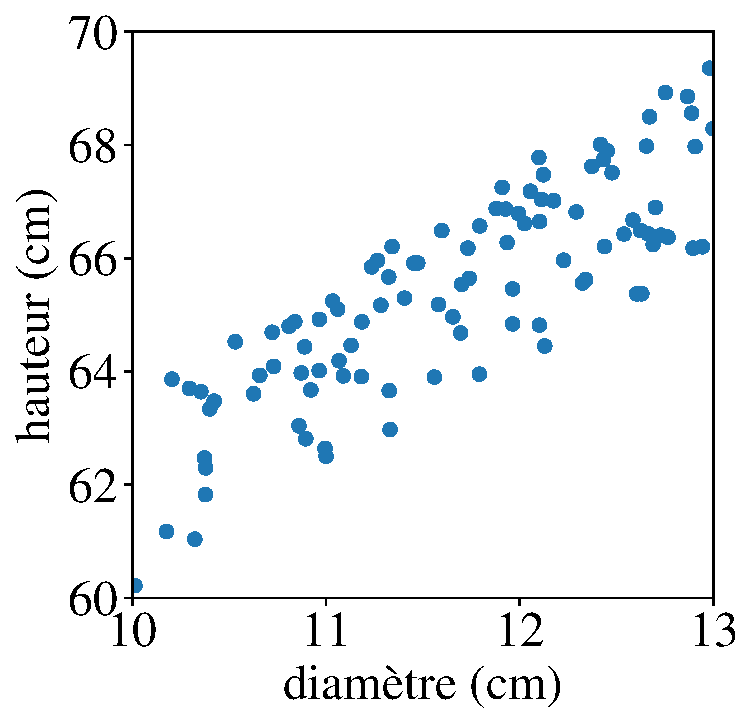
\includegraphics[width=0.35\textwidth]{figures/pearson_example}
\end{center}



\section*{Solution}
{%
\noindent
\rotatebox[origin=c]{180}{%
\noindent
\begin{minipage}[t]{\linewidth}
  \paragraph{Question 1.} Une s�rie de bo�tes � moustaches est plus appropri�e
  pour visualiser la relation entre une variable quantitative (dur�e du s�jour)
  et une variable qualitative (�ge par
  tranches). Cf. figure~\ref{fig:remboursement_rembourses_age}.\newline

\paragraph{Question 2.} $r \approx 0,85.$ On peut voir � la � pente � que la
corr�lation est positive. La situation est interm�diaire entre celle des
figures 2.6(\textsc{C}) $(r=0,50)$ et 2.6(\textsc{D}) $(r=1,00)$. Une
corr�lation de $0,95$ serait plus proche de la figure~\ref{fig:pearson}(\textsc{D}) que de
celle donn�e ci-dessus. Remarquez ici que les donn�es ne sont pas homog�nes, au
sens o� elles ont des �chelles de valeurs diff�rentes, contrairement � ce qui
est repr�sent� sur la figure~\ref{fig:pearson} ; cela ne change pas l'interpr�tation de la
corr�lation.
\end{minipage}%
}%


%%% Local Variables:
%%% mode: latex
%%% TeX-master: "../../sdd_2021_poly"
%%% End:
